%%
%% This is file `sample-sigconf.tex',
%% generated with the docstrip utility.
%%
%% The original source files were:
%%
%% samples.dtx  (with options: `sigconf')
%% 
%% IMPORTANT NOTICE:
%% 
%% For the copyright see the source file.
%% 
%% Any modified versions of this file must be renamed
%% with new filenames distinct from sample-sigconf.tex.
%% 
%% For distribution of the original source see the terms
%% for copying and modification in the file samples.dtx.
%% 
%% This generated file may be distributed as long as the
%% original source files, as listed above, are part of the
%% same distribution. (The sources need not necessarily be
%% in the same archive or directory.)
%%
%% The first command in your LaTeX source must be the \documentclass command.
\documentclass[sigconf,natbib=false]{acmart}

\usepackage[backend=biber]{biblatex}
\usepackage{graphicx}
\graphicspath{ {../calc2/} }
\addbibresource{ref.bib}

%%
%% \BibTeX command to typeset BibTeX logo in the docs

%% Rights management information.  This information is sent to you
%% when you complete the rights form.  These commands have SAMPLE
%% values in them; it is your responsibility as an author to replace
%% the commands and values with those provided to you when you
%% complete the rights form.
\setcopyright{acmcopyright}
\copyrightyear{2018}
\acmYear{2018}
\acmDOI{10.1145/1122445.1122456}


%% end of the preamble, start of the body of the document source.
\begin{document}

\title{Network storage with P4}

%%
%% The "author" command and its associated commands are used to define
%% the authors and their affiliations.
%% Of note is the shared affiliation of the first two authors, and the
%% "authornote" and "authornotemark" commands
%% used to denote shared contribution to the research.
\author{Tamas Lengyel}
\email{d1b5hi@inf.elte.hu}

\author{Noel Hetei}
\email{njoim8@inf.elte.hu}

\author{Peter Kokai}
\email{kokaipeter@gmail.com}


%%
%% The abstract is a short summary of the work to be presented in the
%% article.
\begin{abstract}
Using P4, python and MiniNet our task was to create a network storage which could use any custom topology, given a few constraints. With a simple python client, data could be uploaded, queried and removed from the network. 
\end{abstract}

%%
%% Keywords. The author(s) should pick words that accurately describe
%% the work being presented. Separate the keywords with commas.
\keywords{p4lang, network storage, mininet, bmv2}

%%
%% This command processes the author and affiliation and title
%% information and builds the first part of the formatted document.
\maketitle

\section{Introduction}

P4 introduces a standardized way to data plane programming. It defines how a switch proccesses incoming and outgoing packets. Using python scripting language and MiniNet\cite{mininet}, which creates a virtual network, we created a network storage system where packets are circulating from switch to switch. The goal of the project is to be able to upload, query and remove data from a custom topology using a simple python client. Certain methods and implementation details are going to be described in this paper, along with some of the challenges we faced and how we overcame them.

\section{Overveiw}
In this section we are going show what environment we used to implement the project, and what were the main features we were planning to implement.
\subsection{Preparation}
We used a premade virtual machine environment we found at \textbf{p4lang/tutorials} \cite{p4tut}. Setting up \textit{VirtualBox} with  \textit{Vagrant} tool was required to access the environment. This environment uses the \textbf{P4 v1.0 switch model} \cite{v1model} and the \textbf{BMv2 behavioral model} \cite{bmv2}.
\subsection{Tasks}
Initially, we had the following features in mind for the program:
\begin{itemize}
	\item {\verb|Storing data|}: Where and how to store the incoming data?
	\item{\verb|Implementing operation|}: How to handle incoming operations?
	\item{\verb|Handling Parallel Requests|}: What happens when multiple clients connect?
	\item{\verb|Data Identification|}: How to identify the data?
	\item{\verb|Handling Large Data|}: What happens when large amount of data arrive to a switch?
\end{itemize}

\section{Challenges \& Simplifications}
Each feature has its own challenge. As development went on, we decided to simplify some of these features due to time constraints.
\subsection{Storing Data}
Storing data has raised a lot of questions that had to be considered, for example \textit{What kind of data structure should we use?} and \textit{How the servers positioned in the topology?}. We found that the header is capable of storing data, which was enough for us. We decided to simplify the second question by using only simple topologies where each switch has two or maximum three connections. The data can circulate inside the topology using any port.
\subsection{Implementing Operations}
We decided to implement three operations: \textit{PUT, GET, POP}. Since the clients require some kind of feedback from the server for all of these operations, we had to use package cloning, which became quite a challenge. We decided to \textbf{reserve port 3} in the topology for \textbf{client-server communication} only. This was necessary due to way cloning works: it uses a port that is predefined for the network.
\subsection{Handling Parallel Requests}
Handling multiple request at the same time is hard to implement. One possible solution is to use working queues. Due to time limitations we had to simplify the task so we have assumed that only one user sends data from a single computer into the topology.
\subsection{Handling Large Data}
Large data can be handled server or client side. We have agreed to implement a data size restriction only on the client side. If the users tries to send a data that is larger than the maximum value, the data will not be sent to the server.
\subsection{Unique ID}
In order to maintain consistency and a way for clients interact with the packages in the database, a unique id had to be assigned for each package. We found \textit{hashing} to be the go-to solution.
\section{Methods}
Cloning, id hashing and data forwarding were the most challenging parts of the project.
\subsection{Cloning}
In order to give a response for the clients the data has to be cloned. We use two headers to differentiate between data that are circulating and data that are used to give response or uploaded. Firstly, we clone in the \textit{PUT operation} to send back the a result if the method was succesful. During this operation we copy all the incoming id, and data to the circulating header type. Second time for the \textit{GET operation} becuase if we send back the data that is circulating in the topology we are going to remove it. This operation we follow the same logic that was behind the \textit{PUT operation}, however, we use it in a revesre way. From the header of the circulating data we copy the data into the API header that is responsible for the communication with the clients.
\cite{cloning1} \cite{cloning2}
\subsection{Hashing}
To be able to interact with data and maintain consistency we have given each datum a unique ID that is generated with the built-in CRC16 hashing \cite{hashing2} algorithm. We have used hashing during \textit{ingress} and \textit{egress processing}. First, we check which kind of header is active, then calculating the ID. Hashing has to be implemented twice in the ingress and egress for the two kind of header. As stated above we use cloning to send back data, however the cloned data is not containing the generated ID. In the egress processing we recalculate the hashed id to assign it to the clone.
\cite{hashing1}
\subsection{Forwarding}
To make the data circulating in the given topology we have implemented two tables. One is for handling the different operations, \textit{PUT, GET, and POP}, the second table is for forwarding the messages. We use a boolean variable to mark data on \textit{PUT and GET} operations to be circlulated. The key of the table is the ingress port. If the key is equal to port \#1 or \#3 data is going to be forwarded on port \#2. The only incoming parameter for the actions is the port number where data are going to be forwarded.
\section{Tests \& Results}
For testing we have used a linux virtual machine that has MiniNet pre-installed. To start the project we have to run the \textit{init\_netstore.py} to initialize the port where the communication with the client happens. After that the P4 program can be started. We used a triangle topology to test the program. It has one host and three swicthes all of which are circulating the data using the same port number. Communication with clients happens on port \#3.
\begin{figure}[ht]
	\caption{Topology graphical represenation}
	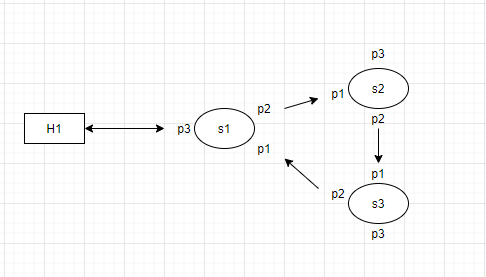
\includegraphics[scale=0.7]{top.png}
	\centering
\end{figure}

\section{Conclusion}
Programing switches can be hard. Our task was to create a network storage in P4 language with the help of MiniNet and python. In the topology the data had to be circulated through switches. Due to time limitations we have simplified some parts of the project, for example: the port where the communication executed with clients is hardcoded. Three operations had to be implemented: \textit{PUT, GET and POP}. The first two used cloning the give proper response to the clients. All data has unique IDs using the built-in hashing algorithm. Looking at the logs show that when puting data in the topology that is circulating through the switches. All things considered, we have achived our goal to store data.

\begin{thebibliography}{2}
\bibitem{p4tut} https://github.com/p4lang/tutorials
\bibitem{mininet} http://docs.mininet.org
\bibitem{v1model} https://github.com/p4lang/p4c/blob/master/p4include/v1model.p4
\bibitem{bmv2} https://github.com/p4lang/behavioral-model
\bibitem{hashing1} https://p4.org/p4-spec/docs/PSA.html\#sec-hash-function
\bibitem{hashing2} https://www.net.in.tum.de/fileadmin/bibtex/publications/papers/2019-P4-workshop-hashing.pdf
\bibitem{cloning1} https://p4.org/p4-spec/docs/PSA.html\#sec-clone
\bibitem{cloning2} http://csie.nqu.edu.tw/smallko/sdn/p4-clone.htm

\end{thebibliography}


%%
%% The next two lines define the bibliography style to be used, and
%% the bibliography file.
%%\printbibliography



\end{document}
\endinput
%%
%% End of file `sample-sigconf.tex'.
